%La fila 2 obliga a que la columna 1 sea celeste, y la fila 3 obliga a que la columna 2 sea verde. Con esa configuración, en la fila 1 deben eliminarse ambas piedras y queda vacía.

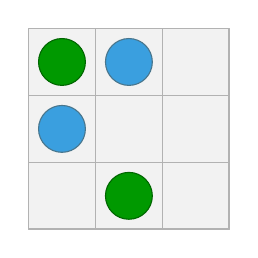
\begin{tikzpicture}[
    scale=0.85,
    transform shape,
    celda/.style={draw=gray!60, fill=gray!10, line width=0.6pt},
    verde/.style={circle, fill=green!60!black, draw=green!40!black, minimum size=0.7cm, inner sep=0pt},
    celeste/.style={circle, fill=cyan!75!blue!80, draw=cyan!50!black, minimum size=0.7cm, inner sep=0pt}
]

\draw[celda] (0,0) rectangle (3,3);
\draw[celda] (0,0) grid (3,3);

% Fila 1 (arriba: y=2.5) -> Verde en col 1, Celeste en col 2
\node[verde] at (0.5, 2.5) {};
\node[celeste] at (1.5, 2.5) {};

% Fila 2 (medio: y=1.5) -> Solo Celeste en col 1 (fuerza col 1 a ser celeste)
\node[celeste] at (0.5, 1.5) {};

% Fila 3 (abajo: y=0.5) -> Solo Verde en col 2 (fuerza col 2 a ser verde)
\node[verde] at (1.5, 0.5) {};

\end{tikzpicture}
